\section{方法}
有别于其他类型的检测问题,如车牌检测和人脸检测,二维码检测有其独特的检测特征——二维码的编码特征。\\
二维码在设计过程中引入的定位模块,修正模块,对齐模块等编码模块都有助于快速准确地检测到二维码的位置。
基于二维码的编码特征,我们实现了两个二维码检测的方法,第一个相对简单直接,第二个针对复杂摄像环境下,对第一个方法做了改进。
\subsection{第一种方法:基础方法}
之所以称为基础方法,是因为这个方法直接利用二维码的编码特征,目的是为了从一幅简单的图片中定位二维码的位置。\\
基础方法的检测步骤如图\ref{fig:basic}所示。
\begin{figure}[h]
\centering
\includegraphics[width=0.9\linewidth]{../../../presentation/basic}
\caption[steps]{基础方法的检测步骤}
\label{fig:basic}
\end{figure}
\subsubsection{转换成灰度图}
为了减小计算量,一般将彩色图像转换成灰度图像。灰度图像与彩色图像一样反映整幅图像的整体和局部的色度和亮度等级的分布和特征。\\
图像的灰度化处理可以用两种方法来实现:(1).以每个像素点的R,G,B三个分量的平均值作为该点的灰度值。(2).根据YUV(亮度,色度,色温)颜色空间和RGB空间的对应关系进行转换,其中Y分量的物理意义是亮度,可以代表图像的灰度等级。利用公式\ref{yuv}可以将彩色图像转换成灰度图像,灰度级别为256,灰度图像中的像素为0~255的亮度值。
\begin{equation}\label{yuv}
Gray = 0.299 * R + 0.5866 * G + 0.1145 * B
\end{equation}
实验采用第二种方法来灰度化原始图像。
\subsubsection{高斯模糊}
对于灰度化的图像,我们采用高斯模糊来去除图像中的噪声,方便之后的轮廓检测。
高斯滤波算法中,分布不为零的像素组成的卷积矩阵与原始图像做变换。
每个像素的值都是周围相邻像素值的加权平均。
原始像素的值有最大的高斯分布值,所以有最大的权重,相邻像素随着距离原始像素越来越远,其权重也越来越小。
这样进行模糊处理比其它的均衡模糊滤波器更高地保留了边缘效果,这样就有利于我们之后的轮廓检测。\\
高斯模糊之后的图像如图\ref{fig:blured}(b)所示。
\begin{figure}[h]
\centering
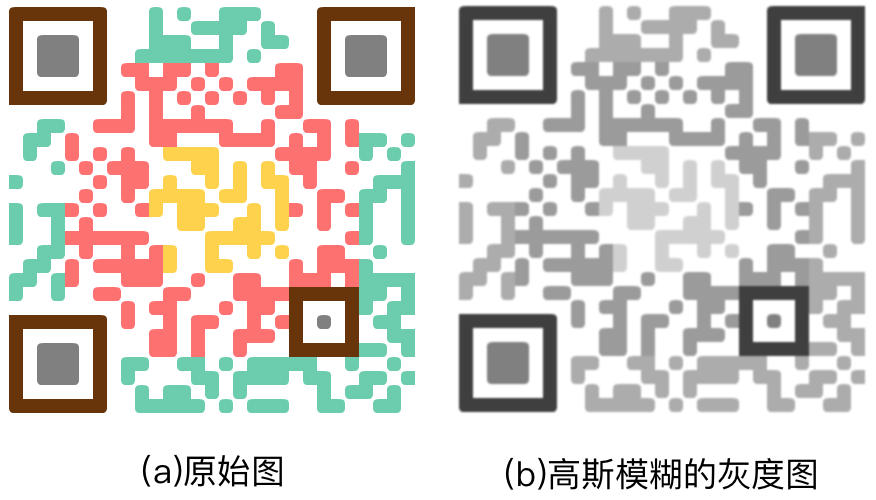
\includegraphics[width=0.9\linewidth]{blured}
\caption[blured]{QR码的原始图和模糊灰度图}
\label{fig:blured}
\end{figure}
\subsubsection{边缘增强}
\subparagraph{Max-Min算法}
通常输入的图像可能包含大量的边缘纹理和噪声信息,Max-Min差分操作\cite{13}能有效减少一些较小的噪声,同时目标区域的效果。
Max-Min差分操作的基本表达式\ref{maxmin1}如下:
\begin{equation}\label{maxmin1}
D(x,y) = max\{f(x+i, y+j)\} - min\{f(x+i, y+j)\}
\end{equation}
其中,$ 0 \le x \le w, 0 \le y \le h $, $ w $ 和 $ h $ 为输入图像的高和宽。\\
\begin{equation}\label{max}
max = max\{f(x+i,y+j)\}
\end{equation}
\begin{equation}\label{min}
min = min\{f(x+i,y+j)\}
\end{equation}
其中,$ 0 \le i \le 3, 0 \le j \le 3 $, $ max $ 和 $ min $ 分别表示输入图像中一个窗口大小为 4*4的区域内像素值的最大值和最小值。\\
经Max-Min操作后二维码区域被较好地突显出来,同时部分噪声也能够得到抑制。这种方法使提取的目标区域,即黑白相间的二维码区域的相邻像素间显示出较高的差异性,这种特性为后续二维码的分割提取提供了很好的保证。
\subparagraph{Canny算子}
边缘提取以及边缘增强是图像处理中的基本方法,Canny算子\cite{14}增强效果明显。
在二维码检测定位的应用中,目标的边缘信息是非常重要的特征之一。
图像边缘保留了原始图像中相当重要的部分信息,同时又使总的数据量减少,这正符合二维码特征提取的要求。\\
Canny算子能够尽可能多地标识出图像中的实际边缘,漏检真实边缘的概率和误检非边缘的概率都比较小。
其检测到的边缘点的位置距离实际边缘点的位置最近。
因此,引入Canny算子作为本实验边缘提取的方法,用于找到二维码的最优边缘。
经过Canny算子增强边缘之后的图像如图\ref{fig:canny}所示。
\begin{figure}[h]
\centering
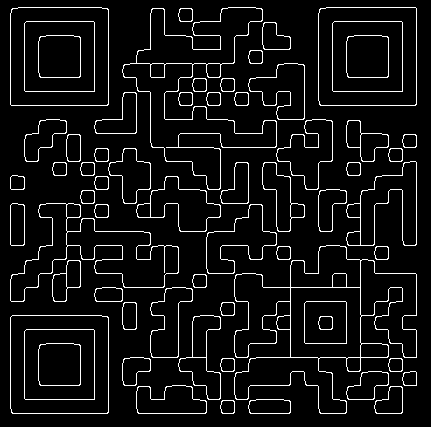
\includegraphics[width=0.5\linewidth]{canny}
\caption[canny]{Canny算子增强边缘后的图像}
\label{fig:canny}
\end{figure}
\subsubsection{轮廓检测}
在上一步得到边缘信息之后,接下来我们通过检测轮廓来找到二维码中的定位模块。\\
在这里我们使用了OpenCV提供的轮廓检测方法:“findfindContours”。
OpenCV中对轮廓采用层次结构的表示方式,如图\ref{fig:contour}示意。
\begin{figure}[h]
\centering
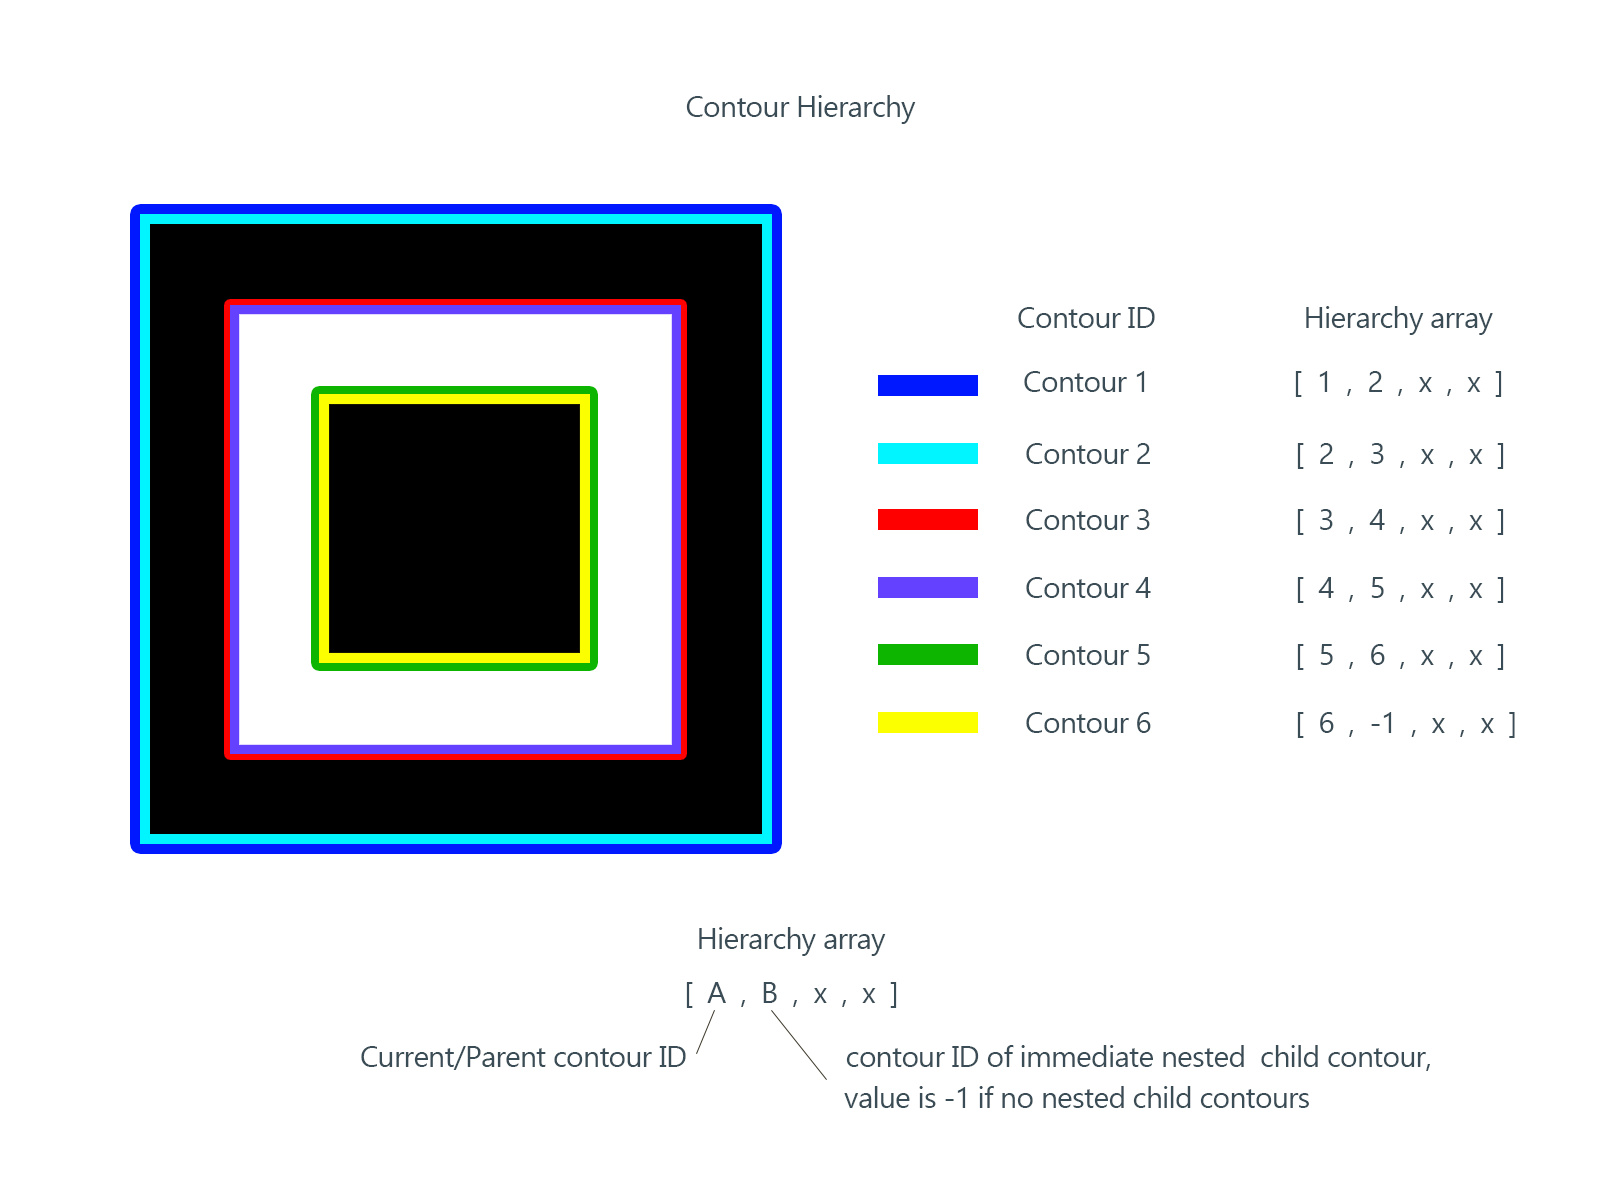
\includegraphics[width=1\linewidth]{contour}
\caption[contour]{OpenCV中轮廓的表示形式}
\label{fig:contour}
\end{figure}
由于这里一条边缘会有内外两条轮廓,所以对于简单的图像,只要遍历轮廓的层次关系,找到嵌套层数大于等于5的轮廓,就是我们要找的定位模块。
图\ref{fig:detection}(a)-(c)即为从图像中找到的定位模块。
\begin{figure}[h]
\centering
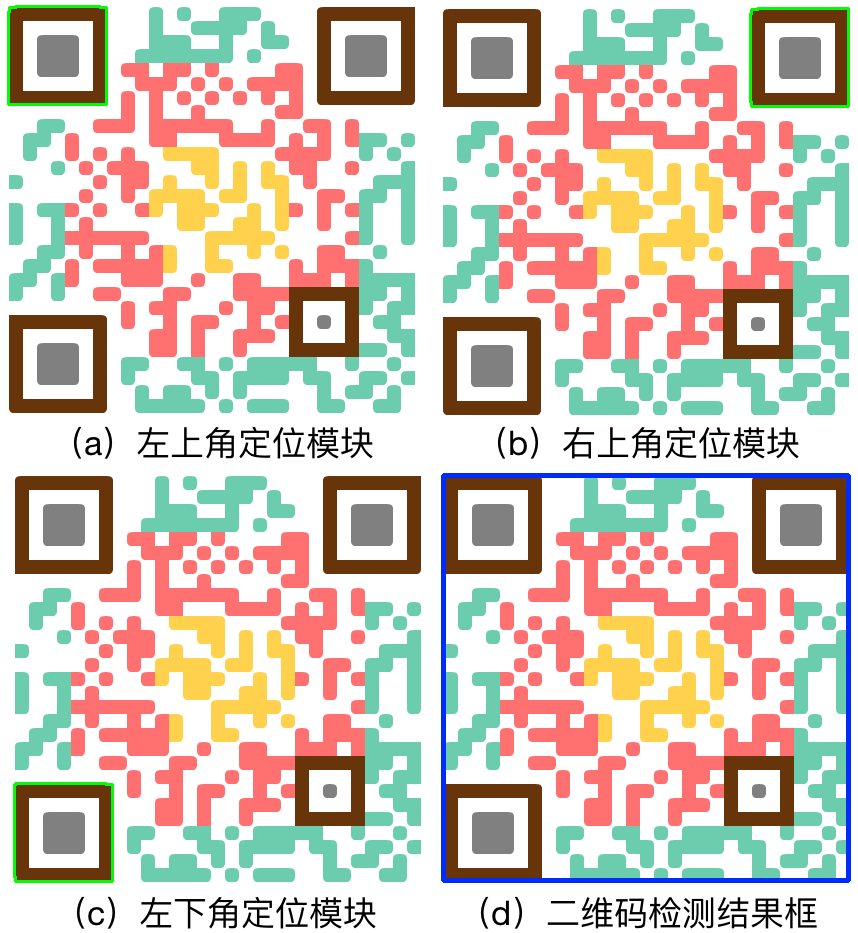
\includegraphics[width=0.9\linewidth]{detection}
\caption[detection]{检测到的QR码定位模块和检测结果框(绿色标记为定位模块,蓝色标记为检测结果框)}
\label{fig:detection}
\end{figure}
\subsubsection{最小区域覆盖}
在规范的二维码中,一旦检测到了三个定位模块,那么整个二维码的结果框就自然而然地形成了。\\
在这里我们使用了OpenCV提供的最小矩形区域方法:”minAreaRect“和包围盒顶点方法:”BoxPoints“。
最小矩形区域方法用来得到覆盖上述三个定位模块的最小矩形,从而将这个最小矩形设置为二维码检测的结果框。
包围盒顶点方法用来得到最小矩形的四个顶点坐标,便于之后将检测结果框绘制出来。\\
利用这两个便利的方法,我们可以得到原始二维码的检测结果框如图\ref{fig:detection}(d)所示。
\subsubsection{优缺点}
\subparagraph{优点}
基本方法的优点在于实现简单明了,检测的速度也有保证,对于拍摄清晰端正,背景简单的图像有较好的检测效果。
\subparagraph{缺点}
另一方面,这类简单方法的缺点也很明显。
(1).对于复杂图像场景下的二维码,检测框可能会跑偏,检测到另外的二维码的定位模块。在实验中,如图\ref{fig:problem1}的二维码场景就会出现误检,将检测框覆盖了其他的二维码的定位模块。
\begin{figure}[h]
\centering
\includegraphics[width=0.7\linewidth]{../../../presentation/problem3}
\caption[problem1]{基本方法的问题:检测框错误覆盖}
\label{fig:problem1}
\end{figure}
(2).当二维码图像在拍摄时因为角度问题产生透视时,基本方法的检测框显得过大,而且检测结果仍是透视的,不便于之后的解码识别操作。图\ref{fig:perspectiveproblem}即是这个问题的具体例子。
\begin{figure}[h]
\centering
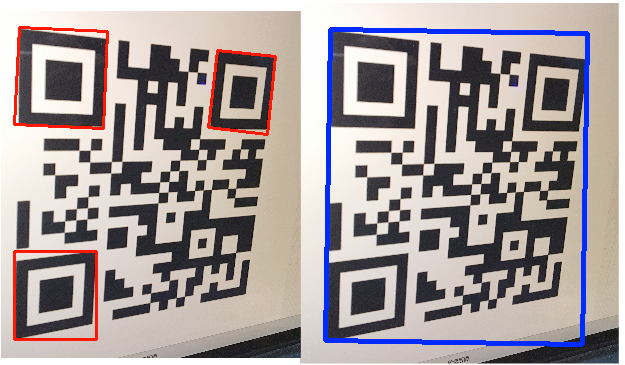
\includegraphics[width=0.9\linewidth]{perspective_problem}
\caption[problem2]{图像透视时的检测问题}
\label{fig:perspectiveproblem}
\end{figure}
\subsection{第二种方法:改进方法}
针对于基本方法的缺点,我们再次基于二维码的编码特征,来改进我们的检测方法,作为实验的第二种方法。
\subsubsection{利用修正模块辅助定位}
在介绍二维码结构的部分,我们介绍了二维码的修正模块,也就是定位模块间一横一竖的两条黑白相间的线。\\
对于类似于图\ref{fig:problem1}中的问题,引入修正模块之后就可以迎刃而解。只有某个二维码本身的定位模块之间,才会有两条修正模块,而与其他二维码的定位模块之间不会存在和修正模块一样的编码模式。利用这个编码特征,我们就可以使用如图\ref{fig:correct}所示的方法来辅助定位。
\begin{figure}[h]
\centering
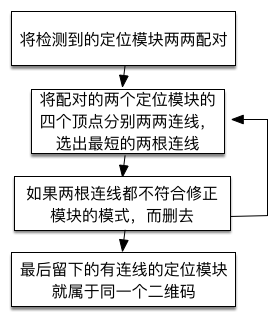
\includegraphics[width=0.8\linewidth]{correct}
\caption[correct]{利用修正模块辅助定位的方法}
\label{fig:correct}
\end{figure}
图\ref{fig:improve1}是所有定位模块两两配对之后选出的配对间最短的两根连线。
\begin{figure}[h]
\centering
\includegraphics[width=0.8\linewidth]{../../../presentation/improve1}
\caption[improve1]{定位模块配对间最短的两根连线}
\label{fig:improve1}
\end{figure}
由二维码的编码可以知道,修正模块是黑白方格间隔分布形成的。由此,我们只要构造出直线遍历器,统计上图所有连线上的黑白像素个数,看统计结果中黑白方格是否均匀分布即可。\\
由统计学知识我们知道,判断分布是否均匀,可以计算数据的方差,方差小意味着数据相近或相同,即黑白方格均匀分布,连线处于修正模块上。
反之,则是黑白方格不均匀分布,连线不在修正模块上。\\
一条典型的修正模块模式的连线上,黑白间隔像素数的统计结果可能是[5,5,6,6,5], 其方差是0.24。\\
而不是修正模块模式的连线上,黑白间隔像素数的统计结果可能是[1,5,9,3,6],其方差是7.36。\\
利用这种方法,我们可以筛选出如图\ref{fig:improve2}的两条位于修正模块上的连线。
\begin{figure}[h]
\centering
\includegraphics[width=0.7\linewidth]{../../../presentation/improve2}
\caption[improve2]{筛选出的位于修正模块上的连线}
\label{fig:improve2}
\end{figure}
进一步地,修正模块连接的三个定位模块就可以确定一个二维码的检测框,如图\ref{fig:improve3}所示。
\begin{figure}[h]
\centering
\includegraphics[width=0.7\linewidth]{../../../presentation/improve3}
\caption[improve3]{修正模块辅助定位得到的检测框}
\label{fig:improve3}
\end{figure}
\subsubsection{利用对齐模块进行反向透视变换}
在设计二维码结构时也考虑到了图像透视问题,所以在其结构中添加了对齐模块。
我们接下来的反向变换就是建立在标识出对齐模块的基础上的。\\
一开始尝试了利用三个定位模块的外顶点作为反向变换的定位点,对变形的图像做反向仿射变换,结果如图\ref{fig:affine}所示。
\begin{figure}[h]
\centering
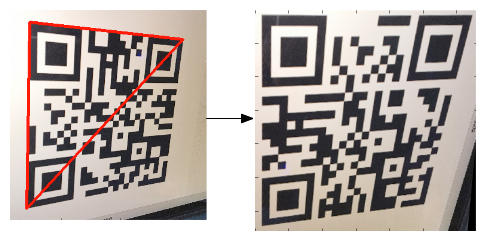
\includegraphics[width=0.9\linewidth]{affine}
\caption[affine]{反向仿射变换}
\label{fig:affine}
\end{figure}
从图中可以看出,反向仿射变换并没有解决图像透视的问题,对于图像规范化的帮助不大。\\
于是自然而然地想到将二维码的对齐模块作为第四个定位点,利用反向透视变换,来得到较为规范的二维码图像。\\
有了之前检测定位模块的经验,检测对齐模块也是同样的道理。不过添加了额外一步,通过检测到的矩形的面积大小来筛选对齐模块,以防止误检。
对图像做反向透视变换的结果如图\ref{fig:propective}所示。
\begin{figure}[h]
\centering
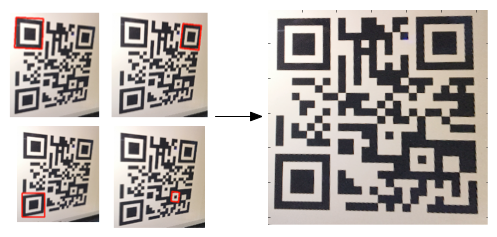
\includegraphics[width=0.9\linewidth]{propective}
\caption[prospective]{反向透视变换}
\label{fig:propective}
\end{figure}
\subsubsection{优缺点}
\subparagraph{优点}
相较于基本方法,能够检测复杂背景下的多个二维码,同时也能很好的处理透视变形的二维码图像。
\subparagraph{缺点}
相较于基本方法,改进方法的计算量较大,实时性的表现较弱。